\documentclass[dvipdfmx, a4p, cjk]{beamer}

% template package
\usepackage{txfonts}
\usepackage{hyperref}
\usepackage{pxjahyper}
\usepackage{bxdpx-beamer}
\usepackage{color}
\usepackage{url}
\usepackage{amsmath, amssymb}
\usepackage{type1cm}
\usepackage{bm}
\usepackage{graphicx}
\usepackage{subfigure}
\usepackage{verbatim}
\usepackage{wrapfig}
\usepackage{multicol}
\usepackage{listings,jlisting}

% my command
\newcommand{\argmax}{\mathop{\rm arg~max}\limits}
\newcommand{\argmin}{\mathop{\rm arg~min}\limits}
\newcommand{\red}[1]{\textcolor{red}{#1}}
\newcommand{\green}[1]{\textcolor{green}{#1}}
\newcommand{\blue}[1]{\textcolor{blue}{#1}}
\newcommand{\cyan}[1]{\textcolor{cyan}{#1}}
\newcommand{\magenta}[1]{\textcolor{magenta}{#1}}
\newcommand{\yellow}[1]{\textcolor{yellow}{#1}}


% beamer
\usetheme{Madrid}
\usecolortheme{dolphin}
\usefonttheme{professionalfonts}
\useinnertheme{circles} 
\setbeamertemplate{navigation symbols}{} % remove navigation
\setbeamertemplate{headline}{%
\leavevmode%
  \hbox{%
    \begin{beamercolorbox}
        [shadow=false, wd=\paperwidth,ht=2em,dp=1.0em]
        {palette tertiary}
        %{palette quaternary}%
    \bf
    \insertsectionnavigationhorizontal{\paperwidth}{\hskip0pt plus1filll}{\hskip0pt plus1filll}
    \end{beamercolorbox}%
  }
}
\newcommand{\inlineframe}[2]{\section{#1}\begin{frame}{#1}#2\end{frame}}

% listing
\lstset{ % color
    backgroundcolor={\color{black}},
    basicstyle={\small \color{white}},
    identifierstyle={\small},
    commentstyle={\small\ttfamily \color[rgb]{0, 0.75, 0}},
    keywordstyle={\small\bfseries \color[rgb]{0.15,0.15,0.85}},
    ndkeywordstyle={\small},
    stringstyle={\small\ttfamily \color{yellow}},
    frame={tb},
    breaklines=true,
    columns=[l]{fullflexible},
    numbers=left,
    xrightmargin=0zw,
    xleftmargin=3zw,
    numberstyle={\scriptsize},
    stepnumber=1,
    numbersep=2.56mm,
    morecomment=[l]{//}
}
% \lstset{ % 白黒
%   basicstyle=\footnotesize\ttfamily, % size of fonts used for the code
%   breaklines=true,                   % automatic line breaking only at whitespace
%   escapeinside={\%*}{*)},            % if you want to add LaTeX within your code
%   keywordstyle=\bfseries,            % keyword style
% }

\title{なんとか年度第n回 \\ HOOBARの会}
\author{Yohei Saito}
\institute[なんとか研究室]{信州大学 理工学科 なんとかかんとか研究室}
\date{日付を忘れないで}

\begin{document}
\frame{\titlepage \thispagestyle{empty}}
\frame{\tableofcontents \thispagestyle{empty}} 

\section{はじめに}
\begin{frame}{はじめてのスライド}
    \begin{definition}
    1と自分自身しか約数を持たない数を\alert{素数}という.
    \end{definition}
    \begin{example}
        \begin{itemize}
        \item 2 は素数.
        \item 3 も素数.
        \item 4 は素数ではない.
        \end{itemize}
    \end{example}
\end{frame}

\section{挿入系スライド}
\begin{frame}{適当な表とソースコード}
\begin{columns}
    \begin{column}{0.4\hsize}
    \begin{table}
    \begin{tabular}{lll}
        hoge & foo & bar \\ \hline
        hoge & foo & bar \\
        hoge & foo & bar \\
        hoge & foo & bar \\
    \end{tabular}
    \end{table}
    \end{column}
    \begin{column}{0.6\hsize}
        \lstinputlisting[language=C++]{hello.cpp}
    \end{column}
\end{columns}
\end{frame}

\begin{frame}{フレームタイトル}
\begin{columns}
    \begin{column}{0.4\hsize}
    内容をここに書く.
    \end{column}
    \begin{column}{0.6\hsize}
    \alert{強調}\\
    \bf{bold}\\
    \sl{naname}\\
    \it{itaric}\\
    数式:$a=b=c$
    \end{column}
\end{columns}

\begin{columns}
    \begin{column}{0.5\hsize}
        \begin{figure}[b]
            \begin{center}
            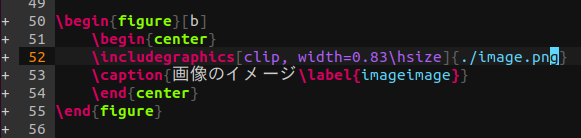
\includegraphics[clip, width=1\hsize]{./img/image.png}
            \caption{画像のイメージ\label{imageimage}}
            \end{center}
        \end{figure}
    \end{column}
    \begin{column}{0.5\hsize}
        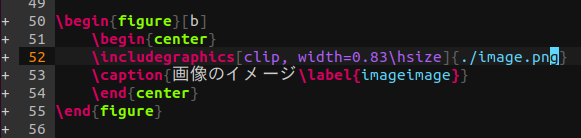
\includegraphics[clip, width=1\hsize]{./img/image.png}

    \end{column}
\end{columns}

\end{frame}


\section{いろいろなスライド}
\begin{frame}{block}
    \begin{block}{This is a block}
        普通のブロック
    \end{block}
    \begin{alertblock}{This is a alert block}
        アラートブロック
    \end{alertblock}
    \begin{exampleblock}{This is a example block}
        example
        $r \neq 0$
        \[ \mathcal{S}' = \{ p \in \mathcal{S} \mid \min_{k_i \in \mathcal{K}} \|p - k_i\| < r_{kpp} \} \]
    \end{exampleblock}
\end{frame}

\inlineframe{テスト}{
    これはインラインフレームです
    \begin{block}{This is a block}
        普通のブロック
    \end{block}
}
\end{document}
